
The Liquid Argon Time Projection Chamber (LArTPC) can be broken down into three major subcomponents: $1)$ The high voltage system which provides the drift field voltage; $2)$ the cathode and field cage which steps down the high voltage through a network of voltage-dividing resistors to form a uniform electric field for charges to drift within; and $3)$ the wire planes which provide the charge sensitive readout for the detector. Here we describe each of the subcomponents which make up the LArIAT LArTPC.

%%%%%%%%%%%%%%%%%%%%%%%%%%%%%%%%%%%%%%%%%%%%
\begin{subsubsection}{High Voltage}\label{sec:DriftVoltage}
%%%%%%%%%%%%%%%%%%%%%%%%%%%%%%%%%%%%%%%%%%%%
The drift high voltage system for the LArIAT detector, shown pictorially in Figure~\ref{fig:HVScheme}, is designed to allow ionization electrons from the interaction of charged particles in the liquid argon to drift to the wireplanes. The high voltage system consists of a Glassman LX125N16 power supply~\cite{GlassmanPS} capable of generating -125~kV and 16~mA of current. This power supply was typically operated much below this limit during normal data taking operations. The voltage from the power supply is transmitted through high voltage cables to a series of filter pots before finally reaching the high-voltage feedthrough on the top of the LArIAT cryostat. This feedthrough brings the voltage into the liquid argon volume to be transmitted to the TPC cathode.


\begin{figure}[htb]
\centering
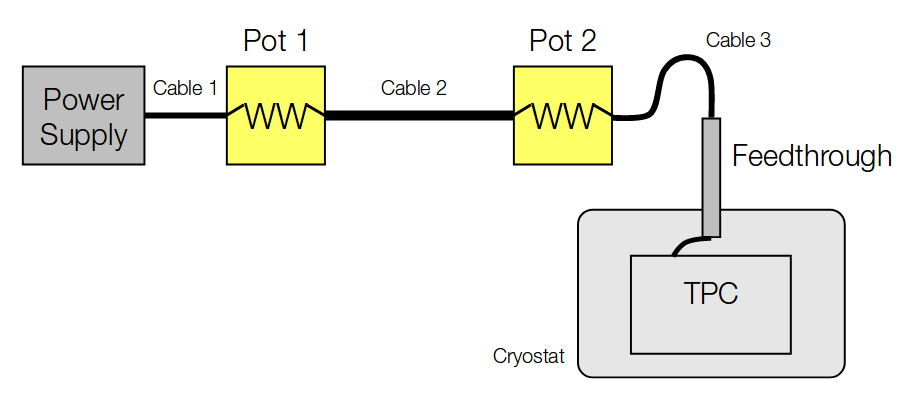
\includegraphics[scale=0.35]{./figures/HVSchematic.png}\\
\caption{Schematic of the LArIAT high voltage system.}
\label{fig:HVScheme}
\end{figure}%See DocDB 1472

The first high voltage cable which connects the Glassman power supply to the first filter pot is a 1/2-inch HV cable, Glassman cable model 2121, supplied by the Glassman manufacturer. The second cable is a $\sim$100-ft long 1/2-inch Type-2134 Dielectric Sciences cable which connects the first filter pot to the second filter pot. Finally, the same type of cable is used to connect the second filter pot to the high voltage feedthrough at the cryostat.

The two filter pots that are inline with the high voltage system serve to: $a)$ limit the current draw on the power supply; $b)$  provide a low-pass filter to help reduce the voltage ripple on the cathode; and $c)$ partition the energy stored in the system in the event of a high voltage trip. Each filter pot, as shown in Figure~\ref{fig:FilterPot}, is a cylindrical aluminum pot 18.5 inches tall by 20 inches in diameter and 3/16 inches thick, with welded tops each having an opening that allows for a flange and o-ring to receive the high voltage cables. Within each pot, the flanges are connected to four 10~M$\Omega$ resistors connected in series. This assembly is submerged in $\sim$16 gallons of Diala transformer oil~\cite{ShellDiala} to aid in the suppression of corona and discharges.

\begin{figure}[htb]
\centering
\includegraphics[scale=0.35]{./figures/FilterPot.png}\\
\caption{Filter pots used in the LArIAT high voltage system.}
\label{fig:FilterPot}
\end{figure}%See DocDB 1472

The final piece of the high voltage system is the high voltage feedthrough which delivers the drift voltage to the cathode of the TPC. This feedthrough is based on a a custom design that was used by ICARUS \cite{IcarusDetector}. The feedthrough consists of a stainless steel inner conductor surrounded by a tube of ultra high molecular weight polyethylene further surrounded by a stainless steel outer ground tube. The high-voltage feedthrough enters the cryostat from a dedicated 4-5/8 inch Conflat flange at the top of the cryostat. The end of the inner conductor is finally attached to the cathode by a flexible conductor bolted at both ends. A technical drawing of the LArIAt high voltage feedthrough can be found in Figure \ref{fig:HVFT}. 

\begin{figure}[htb]
\centering
\includegraphics[scale=0.35]{./figures/lariatFeedthrough.pdf}\\
\caption{Technical drawing of the LArIAT high voltage feedthrough. Various liquid argon levels are shown in cyan to indicate the levels to ensure the feedthrough is immersed in argon during operations}
\label{fig:HVFT}
\end{figure}%See DocDB 1472

During usual operations, the operating voltage from the Glassman power supply was -23.5~kV corresponding to a drift field of $\sim$500 V/cm. During special runs, the high voltage system was operated in a range from 0~kV to 32.8~kV (corresponding to drift fields ranging from 0~V/cm to 700~V/cm) and the feedthrough was tested up to 60~kV with no electrical breakdown observed.


\end{subsubsection}

%%%%%%%%%%%%%%%%%%%%%%%%%%%%%%%%%%%%%%%%%%%%
\begin{subsubsection}{Cathode and Field Cage}\label{sec:FieldCage}
%%%%%%%%%%%%%%%%%%%%%%%%%%%%%%%%%%%%%%%%%%%%

\textcolor{red}{Description of the cathode and field cage is missing}

As shown in Figure \ref{fig:driftregions}, the LArIAT TPC has three drift volumes, each of which has its own electric field. The main drift volume is defined as the region between the cathode plane and the shield plane (C-S). Note that the shield plane wires are \emph{not} read out. The other two drift regions are those between the shield plane and the induction plane (S-I), and between the induction plane and the collection plane (I-C). The electric field in these regions is chosen to satisfy the charge transparency condition to allow for 100$\%$ transmission of the drifting electrons through the shield and then the induction planes. We provide a detailed description of the electric field measurement in each region in \ref{sec:EFieldMeasurements}.

\begin{figure}[htb]
\centering
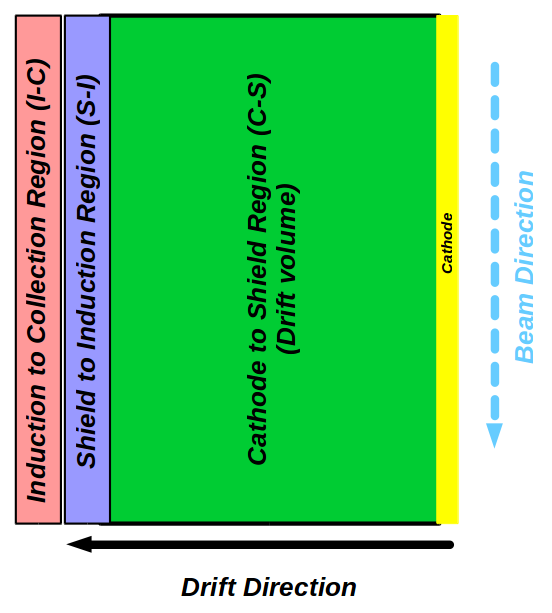
\includegraphics[scale=0.35]{./images/DriftRegions.png}\\
\caption{Schematic of the three drift regions inside the LArIAT TPC: the main drift volume between the cathode and the shield plane (C-S) in green, the region between the shield plane and the induction plane (S-I) in purple, and the region between the induction plane and the collection plane (I-C) in pink.}
\label{fig:driftregions}
\end{figure}

Table \ref{tab:voltages} provides the default voltages applied to the cathode and the shield, induction, and collection plane for all the runs. These voltages were tuned to maintain the transparency condition when the (I-C) and (S-I) spacing changed. For data taken in Run-I, Run-II, and Run-IIIb the spacing was a constant 4~mm; the spacing was 5~mm for Run-IIIa. 

\begin{table}[htpb]
\centering
\caption{Anode planes default voltages}
\label{tab:voltages}
\begin{tabular}{lllll}
\hline
\multicolumn{1}{|l|}{V Cathode} & 
\multicolumn{1}{|l|}{V Shield} & \multicolumn{1}{l|}{V Induction} & \multicolumn{1}{l|}{V Collection} & \multicolumn{1}{|l|}{Run} \\ \hline
\multicolumn{1}{|l|}{-23.17 kV} &
\multicolumn{1}{|l|}{-298.8 V} & \multicolumn{1}{l|}{-18.5 V}      & \multicolumn{1}{l|}{338.5 V} & \multicolumn{1}{|l|}{Run-I, Run-II \& Run-IIIb}      \\ \hline
\multicolumn{1}{|l|}{-23.17 kV} & 
\multicolumn{1}{|l|}{-325.8 V} & \multicolumn{1}{l|}{-0.6 V}      & \multicolumn{1}{l|}{421.9 V} & \multicolumn{1}{|l|}{Run-IIIa}      \\ \hline

                              &                                 &                                 
\end{tabular}
\end{table}

\end{subsubsection}

%%%%%%%%%%%%%%%%%%%%%%%%%%%%%%%%%%%%%%%%%%%%
\begin{subsubsection}{Wire Plane Assembly}\label{sec:WirePlanes}
%%%%%%%%%%%%%%%%%%%%%%%%%%%%%%%%%%%%%%%%%%%%

%%%%%%%%%%%%%%%%%%%%%%%%%%%%%%%%%%%%%%%%%%%%
\begin{subsubsection}*{Wire Winding}
%%%%%%%%%%%%%%%%%%%%%%%%%%%%%%%%%%%%%%%%%%%%

Wires for the LArIAT wire planes are wound to the correct spacing and tension on an independent winding machine before being transferred to the printed circuit boards on which they are installed in the TPC.

\begin{figure}[h!]
\centering
\includegraphics[height=2in]{figures/MamaBear.jpg}
\caption{The wire-winding apparatus in action. Both frames are attached and a single wire has been wound.}
% CAN PROBABLY FIND A BETTER PICTURE!
\label{pic:mamabear}
\end{figure}

Two rectangular steel frames are bolted back-to-back on an apparatus that rotates at a constant speed, shown in Figure \ref{pic:mamabear}. As the frames rotate, wire is drawn from a spool and wrapped around the two frames at constant tension (monitored by a tensiometer in the device paying out the spool). Once the requisite number of wires have been wound, the wires are epoxied onto the steel frames with five-minute epoxy and cut, giving two separate wire planes (one on each frame).
\end{subsubsection}

%%%%%%%%%%%%%%%%%%%%%%%%%%%%%%%%%%%%%%%%%%%%
\begin{subsubsection}*{Wire Transfer}
%%%%%%%%%%%%%%%%%%%%%%%%%%%%%%%%%%%%%%%%%%%%
Once the wire planes have been wound, they must be transferred from the winding frames onto the G10 wire-carrier boards that go into the LArIAT TPC. To achieve this, the frames are unbolted from the winding apparatus and laid over the board onto which the wires are to be transferred, which itself is bolted to a rigid aluminium frame to prevent it from flexing under tension. Careful manual alignment is performed, using guide holes drilled in the board for reference. This alignment is shown in Figure \ref{pic:wiretransfer}.

Once the wires are aligned to the solder pads on the board, they are glued to the board behind the solder pads with a temporary epoxy strip (using five-minute epoxy) to preserve the alignment. This is then followed by a permanent epoxy strip on the inside of the solder pads, using a slow-curing epoxy that is safe for cryogenic conditions. This epoxy is allowed to cure for 12 to 24 hours before the wires are cut behind the temporary strip and the winding frame can be removed.

\begin{figure}[h!]
\centering
\includegraphics[height=2in]{figures/WireTransfer.jpg}
\caption{One of the \textcolor{red}{This can be 4mm or 5 mm wire plane} 3~mm wire planes during transfer, with the wires not yet cut from the winding frame. A steel bar was used for this plane to ensure all wires made good contact with the board.}
\label{pic:wiretransfer}
\end{figure}

\end{subsubsection}

%%%%%%%%%%%%%%%%%%%%%%%%%%%%%%%%%%%%%%%%%%%%%%%%%%%%%%%%%%%%%%%%%
\begin{subsubsection}*{Soldering of Electrical Connections}
%%%%%%%%%%%%%%%%%%%%%%%%%%%%%%%%%%%%%%%%%%%%%%%%%%%%%%%%%%%%%%%%%

When the wire transfer is complete, the wires are soldered to their pads using [SOLDER DETAILS HERE], as are the resistor and capacitor components for the U and V planes \textcolor{red}{Which are the values of capacitances and resistances?}. Mylar sheeting is used to protect the active region of the wire planes from evaporating solder flux during this process. Once all wires have been soldered in place, the wires are broken off behind the solder pads and the temporary epoxy strip is removed. The entire board is cleaned with ethyl alcohol to remove any residue of solder flux before the finished wire planes ahead of installation in the TPC.
\end{subsubsection}

%%%%%%%%%%%%%%%%%%%%%%%%%%%%%%%%%%%%%%%%%%%%%%%%%%%%%%%%%%%%%%%%%
\begin{subsubsection}*{Wire Plane Testing}
%%%%%%%%%%%%%%%%%%%%%%%%%%%%%%%%%%%%%%%%%%%%%%%%%%%%%%%%%%%%%%%%%

\textbf{Electrical Testing}\\
\textcolor{red}{Both the test on the RC and on the wire tension are very bad described. According to me it is better to delete the section if a better description can not be provided.}
Every channel on each completed plane is probed with a multimeter and a signal generator to check for electrical continuity, and in the case of the U and V planes, for the correct RC time constant from the components.\\
\textbf{Tension Testing}\\
A laser tensiometer is mounted on a rigid aluminium arm over each completed frame and used to verify the tension on a representative sample of the wires. [QUANTITATIVE RESULTS?]

\end{subsubsection}

\end{subsubsection}


\textcolor{red}{The title says "Cold" but all the electronic, cold and warm, is described}
The LArIAT TPC front-end electronics comprises a 480-channel analog signal path from the TPC wireplanes to the signal digitizers. The front-end system also includes a digital control system for the TPC-mounted electronics, a power supply, and a distribution system.
A block diagram of the overall system is shown in Fig. \ref{pic:FEelectronics}.

\begin{figure}[htbp]
 \centering
 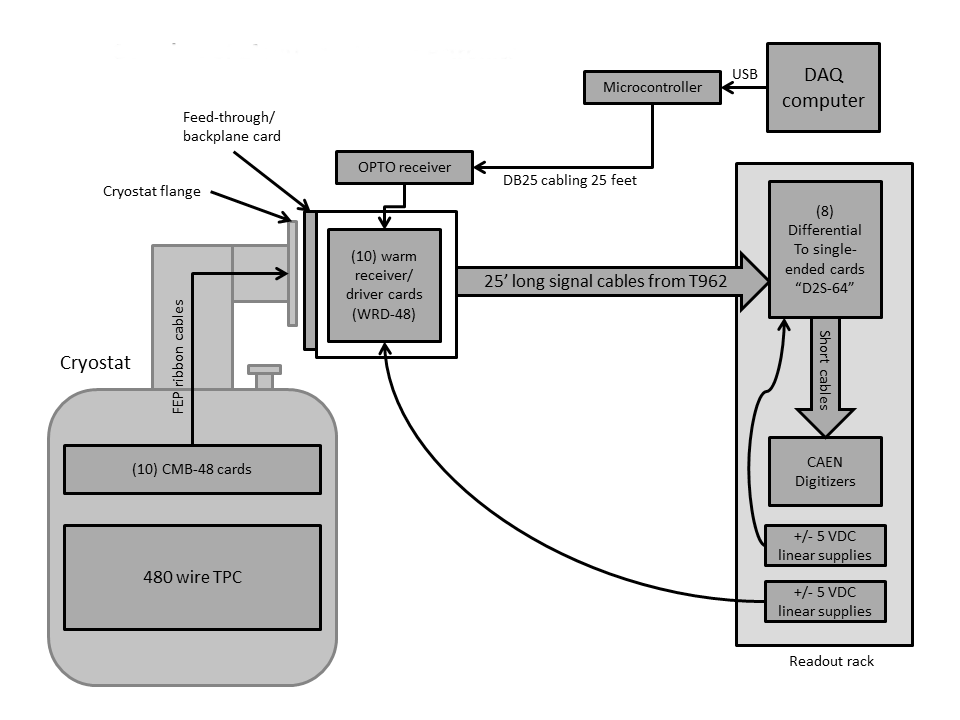
\includegraphics[width=1.0\textwidth]{figures/LArIAT_FE_Electronics.png}
\caption{
Overview of LArIAT Front End electronics. 
} 
\label{pic:FEelectronics}
\end{figure}

The electrical signals on the TPC readout wires are typically quite small, being a direct readout of the ionization of the liquid argon. To achieve a good Signal-to-Noise Ratio (SNR) for such signals, the LArIAT TPC is instrumented with cold amplifiers developed by Brookhaven National Lab (BNL) and mounted directly to the TPC frame inside the liquid argon cryostat. The BNL amplifiers are built as custom Application-Specific Integrated Circuits (ASICs) [ADD reference]. The BNL ASICs adopted in LAriAT are designated as LArASIC, version 4-star.

The LArASICs are mixed signal devices, where the analog amplifier characteristics are controlled by digitally-set parameters. The maximum gain setting of the LArASIC is 25 mV/fc. At this gain a 3.5~fC charge deposition - corresponding to the expected charge arriving at an individual wire from a passing MIP energy deposition - on a readout wire will generate an output with 90~mV amplitude. At the other end of the readout chain, the CAEN V1740 [\textbf{ADD}: CAEN refernece] digitizers have a 12 bit resolution and a maximum input range of 2~VDC, yielding about 0.5~mV LSB. With the analog signal path from LArASIC to the digitizers being designed to provide unity gain, a passing MIP in the TPC is expected to generate a digital signal with amplitude of about 180 ADC counts.  [\textbf{UPDATE}: Dean found gain to be less than unity, add details; what was the measured MIP amplitude?] \textcolor{red}{what is the sampling rate of the board?}

The readout racks containing the signal digitizers are positioned at a distance of $\sim$8~mt from the cryostat and are referenced to a different ground respect to the TPC electronics ground.  The distance minimizes the presence of secondary, tertiary and halo charged particles passing through the digitial electronics.  To prevent problems caused by differing grounds and noise pick-up along the signal transmission line, the single-ended analog signals from the ASICs are transmitted from the cryostat to the readout racks as differential analog pairs, each pair individually shielded.  This is achieved using four types of interconnected cards.  The first type of card in the system is a 48-channel cold motherboard (CMB-48) that mounts directly to the TPC and houses three 16-channel LArASICs per card.  The next card in the signal path is a single cryostat feed through card (FT) that carries the 480 signals, along with power and control lines, across the cryostat boundary.  A set of warm receiver and driver (WRD-48) cards plug directly into the cryostat feed-through and amplify the single-ended TPC signals as differential analog. The differential analog signals are then driven through 8~mt high quality pleated foil cables to a set of differential-to-single-ended (D2S-64) cards, converting the differential signals into single-ended ones, with enough drive capability to allow direct input into an array of CAEN V1740 digitizers.

At the receiving end of the differential path the differential-mode analog signal arrives with common-mode noise cancelled and converted to single-ended analog for the short distance transmission to the CAEN V1740 digitizers.

%%%%%%%%%%%%%%%%%%%%%%%%%%%%%%%%%%%%%%%%%%%%%%%%%%%%%%%%%%%%
\subsection*{Cryostat feed through}
%%%%%%%%%%%%%%%%%%%%%%%%%%%%%%%%%%%%%%%%%%%%%%%%%%%%%%%%%%%%
The feedthrough (FT) card developed for LArIAT is sandwiched between an ASA flange and cap, and sealed with o-rings. A stiff mechanical structure and backplane-style connectors support the FT card and allow for the WRD-48 cards to be plugged directly into it. Such an arrangement facilitates the assembly and potential repair work while reducing the amount of cables and connectors needed.

\begin{figure}[htbp]
 \centering
 \includegraphics[width=0.5\textwidth]{figures/FT_drawings.png}
\caption{
Drawing of LArIAT feed through and Warm Receiver Driver crate. 
} 
\label{pic:FeedthroughElectronics}
\end{figure}

The FT card is built as an 8-layer PCB with dimensions 254~mm $\times$ 432~mm. The outer layers of the card are mostly uninterrupted ground planes to increase noise immunity. The internal traces are built with relatively large 12~mil design rules to enhance manufacturing yield and physical robustness. Signal on adjacent layers are staggered to reduce capacitive cross-talk couplings, and ground fills are provided whenever possible on all copper layers.

Supporting the FT card is a mechanical structure that is rooted on the cryostat flange. The overall assembly of the card, the ten WRD-48 cards, and the WRD card cage is light enough to be safely cantilevered from the cryostat flange. The backplate of the structure is a solid copper sheet which is electrically connected with the cryostat flange though lock washers and also connected to the FT card through 40 conductive standoffs. The copper plate and the cryostat flange are defined as the electrical ground of the TPC readout electronics.

%%%%%%%%%%%%%%%%%%%%%%%%%%%%%%%%%%%%%%%%%%%%%%%%%%%%%%%%%%%%
\subsubsection*{CMB-48 card details}
%%%%%%%%%%%%%%%%%%%%%%%%%%%%%%%%%%%%%%%%%%%%%%%%%%%%%%%%%%%%
Each CMB-48 card holds 3 LArASICs. The card provides electrical connection to the LArIAT TPC wires and mechanical connection to the TPC structure. The CMB-48 board is located inside the cryostat and is thus inaccessible during data-taking periods. The board is designed to minimize the source of electrical noise, the risk of failure due to thermal stress, and the risk of component failure.

%%%%%%%%%%%%%%%%%%%%%%%%%%%%%%%%%%%%%%%%%%%%%%%%%%%%%%%%%%%%
\subsubsection*{WRD-48 card details}
%%%%%%%%%%%%%%%%%%%%%%%%%%%%%%%%%%%%%%%%%%%%%%%%%%%%%%%%%%%%
The WRD-48 cards are designed to be paired one-to-one with the CMB-48 cards inside the cryostat.The WRD-48 cards hold 48 channels of single-ended to differential analog amplifiers to transmit the TPC signals to the distant digitizers. These cards also provide low-noise power regulation, digital signal conditioning, front-panel diagnostic LEDs and voltage monitor ports, and an on-board test-pulse generator. 

%%%%%%%%%%%%%%%%%%%%%%%%%%%%%%%%%%%%%%%%%%%%%%%%%%%%%%%%%%%%
\subsection*{D2S-64 card details}
%%%%%%%%%%%%%%%%%%%%%%%%%%%%%%%%%%%%%%%%%%%%%%%%%%%%%%%%%%%%
The D2S-64 cards convert the differential analog signals from the WRD-48 cards to single-ended signals and drive these signals into the $50 \Omega$ input impedance of the CAEN V1740 digitizers.

The LArIAT data acquisition system is triggered to read out the digitizing buffers by a CAEN V1495 module. The V1495 is a powerful, easily configurable coincidence module featuring a user-programmable FPGA.  Sixteen logical inputs (upgraded to 32 in Run-III) are sampled on a 10~ns clock, checking for matches to any of the sixteen user-defined patterns in the trigger menu.  If a given trigger pattern is satisfied for two consecutive clock ticks, that pattern fires. 

NIM-standard logic pulse inputs to the trigger decision come from any of the instruments in the experiment, in principle; trigger inputs are derived from beam instruments, from the cosmic ray taggers, and from the cryostat's scintillation detectors. LArIAT takes full advantage of the trigger card's great flexibility.  As conditions change and innovations are gradually made to LArIAT's data-taking process, improvements are made to the trigger input designs and the combinations of inputs which define trigger patterns for the V1495.  The configuration of the trigger inputs is automatically logged in a database at the start of each run as part of the DAQ configuration, along with the rest of the XML configuration file for the V1495.

\subsubsection{Inputs to the Trigger System}

Two primary inputs to the trigger card are from the time of flight (see Sec.~\ref{sec:TOF}) and the wire chamber (see Sec.~\ref{sec:MWPC}) systems in the tertiary beamline.  Coincidence of activity in both of these systems strongly suggests that a charged particle has made the journey down the tertiary beam line from the copper target to the LArTPC in the cryostat, and that we will have a measure of its momentum and its velocity. PMT pulses from the time of flight system each pass through a 
%FIXME WHAT MODEL linear fanout?
linear fan-out, one output of which is threshold discriminated by a
%FIXME WHAT MODEL
discriminator to produce a NIM logic pulse for use in trigger logic.  On each of the upstream or downstream TOF paddles, we form a coincidence to within 20~ns of pulses from all the PMTs observing that same block of scintillator.  The upstream paddle coincidence signal is delayed 20~ns to allow any approximately lightspeed particles to travel 6.5~m to the downstream paddle.  The same upstream paddle coincidence signal is also widened to 100~ns to allow for slow-traveling (high-mass) particles.  Coincidences of these upstream and downstream TOF trigger input signals can be made in the V1495 trigger card.

Each wire chamber is read out by four multi-hit TDCs (time to digital converters), with sixty-four wires per TDC and two TDCs per plane (one horizontal and one vertical).  The TDCs each provide a logical ``fast'' OR of their inputs, indicating that one or more of their sixty-four wires went over the settable threshold.  Using NIM logic units, the OR of the horizontal wires and the OR of the vertical wires are input to a coincidence unit for each wire chamber, providing a single logical pulse for each of the four wire chambers, indicating that at least one horizontal wire and one vertical wire saw significant signal.  The single culminating logical pulses from each of the four wire chambers make up the first four inputs to the V1495 trigger card.  Within the user-programmable FPGA, the V1495 looks for the coincidence within 20~ns of at least three of these four specially-treated logical inputs.

Another primary input to the trigger card is from the cosmic towers (see Section~\ref{sec:CosmicRayPaddle}). To capture cosmic ray events in which a minimally ionizing cosmic ray muon crossed the TPC along the body diagonal, NIM modules form the logical coincidences from the two cosmic towers, one upper and one lower paddle assembly, in each combination.  The OR of these is provided as an input to the V1495. 

Three important logic pulses are derived from the timing of the beam.  These include a pulse in a brief window before the beam, a pulse indicating that the beam is on, and a pulse which defines the beam-free period which may be used for collecting cosmic-ray events.  An adjustable pulser is a fourth trigger input which does not depend on any particular activity in the experiment hall,  useful for collecting background events with zero bias. 

The PMTs observing liquid argon scintillation light (see Section \ref{sec:PhotonSystem}) produce pulses which form the foundation of several interesting trigger inputs.  Thresholding a copy of each PMT pulse (after amplification), and requiring a coincidence of pulses within $\sim$20~ns, creates simple trigger inputs indicating ionizing radiation was produced in the TPC.  This scintillation logic pulse is used to initiate a gate which spans the length of the TPC drift time, creating a logic signal which is remains ``on'' while significant drift charge may still be present in the TPC.  In addition, requiring a delayed coincidence of two subsequent scintillation logic pulses, separated by a variable length of time ranging from 300~ns to 7~$\mu$s, is used to create a trigger input to select events where a cosmic muon stops and decays to a Michel electron in the TPC.  A few different versions of this light-based trigger were implemented throughout the course of LArIAT's run time to allow reconstruction and calorimetric studies of Michel electrons. Figure~\ref{michel_logic} shows a schematic diagram of the logic comprising the Michel electron trigger. 

\begin{figure}
\includegraphics[width=\textwidth]{figures/trigger_michellogic.png}
\caption{\label{michel_logic}A schematic diagram of the trigger logic used to select Michel electron events during the cosmic readout window of the LArIAT supercycle.  The two PMT signals refer to the Hamamatsu (``HMM'') and ETL PMTs described in Section~\ref{sec:PhotonSystem}.  For some data-taking periods in Run-II, un-amplified pulses were discriminated at 180 mV to act as a veto on events that may saturate the dynamic range of the V1751 digitizer.  The discriminator thresholds used on the amplified (x10) PMT signal copies (\emph{ThA}, \emph{ThB}) as well as the Gate Delay period, were adjusted between run periods while experimenting with different configurations.}
\end{figure}

Further trigger inputs come from the beam line instrumentation behind the LArTPC cryostat, the PMTs of the Punch-Through scintillator paddles and those of the scintillator paddles instrumenting the Muon Range Stack.  The PMT pulses of all four of the broad-faced Punch Through paddles are discriminated to form logic pulses.  A single logic pulse is formed from these, indicating activity in at least two overlapping paddles at the rear of cryostat, before the steel block of the range stack.  PMT pulses from the Muon Range Stack are amplified and threshold discriminated.  These MuRS paddle pulses are then combined as in the Punch Through, creating single-bit indicators for each of the four instrumented layers that at least one pair of overlapping scintillator paddles sent signals within a 20~ns coincidence window.

\subsubsection{Trigger Decision and Issuance}

The V1495 may be configured to have up to sixteen trigger patterns and sixteen veto patterns, based on the trigger input signals.  A trigger pattern is defined as the AND of one or more defined inputs, and may include the NOT of the AND of further inputs.  Veto patterns are independently defined in the same way, but they have a very different effect.  When any of the trigger patterns fire, a ``fast trigger'' signal is issued and an adjustable countdown is initiated.  If the countdown completes without a veto pattern firing, the ``slow trigger'' signal is also issued and on a distinct hardware channel. Otherwise, if a veto pattern fires during the countdown, the slow trigger signal is vetoed.  

The fast trigger signal prompts readout of all the `short' data buffers, which include the V1751 modules, the V1495 itself, and the MWPC controller.  The V1751 buffers typically contain digitized PMT signals from the time of flight and cryogenic light collection detectors. Readout of the TPC wire signals, which are much longer and more numerous, is only prompted at the issuance of the slow trigger.


\subsection*{Signal Digitization}

Signals from all photodetectors are routed from the side-flange of the cryostat to NIM fan-outs to provide the 50-Ohm termination needed to minimize reflections along the cables. Copies of the PMT signals are made to aid in several light-based triggers, and copies of all signals are then recored into data using CAEN V1751 digitizer boards with 1~GHz sampling rate.

%------------------------------------------
\begin{figure}
\centering
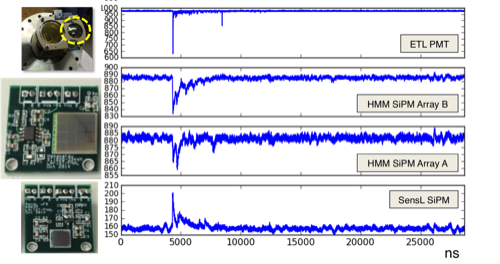
\includegraphics[width=0.8\textwidth]{figures/lightsys_signals.png}
\caption{Some example signals, in ADC units, from LArIAT photodetectors for a triggered cosmic Michel electron event.}
\label{lightsys_signals}
\end{figure}
\begin{figure}
\centering
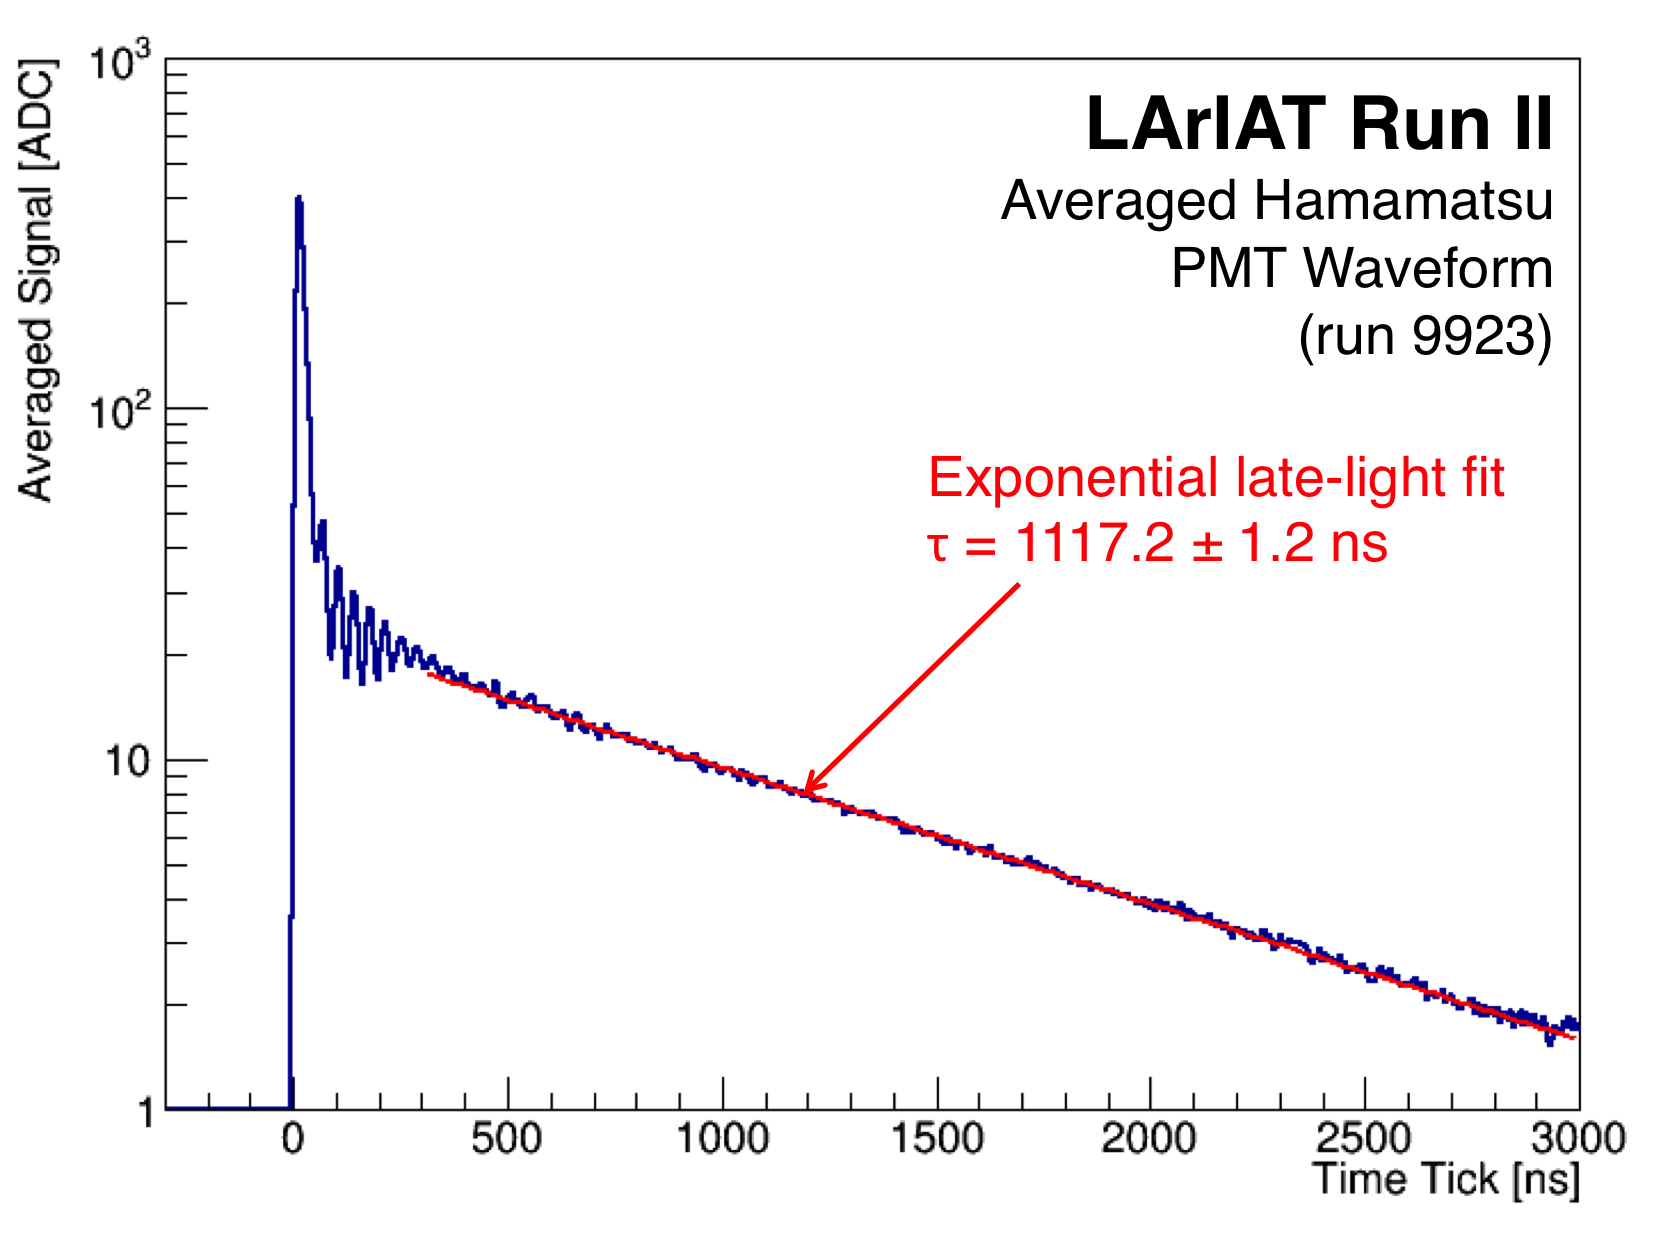
\includegraphics[width=0.6\textwidth]{figures/lightsys_avewfm_hmm.png}
\caption{\label{wfm_hmmpmt}An example of an averaged inverted waveform of the Hamamatsu PMT after event-by-event noise removal and overshoot correction.  Data was taken from a small subset of events from Run-II.  In this example, a falling exponential is fit to the signal region from 300~ns to 3~$\mu$s following the onset of the pulse to extract the late-light component lifetime $\tau$ = 1117~ns.}
\end{figure}
%------------------------------------------

\subsection*{Nitrogen Contamination Measurement Using Light}

The light detection system can also be used to derive information about the nitrogen (N2) contamination in liquid argon. The influence of N2 on liquid argon scintillation light emission has been observed in the WArP experiment~\cite{WARP-nitrogen}. With a higher N2 concentration, the observed decay time of the liquid argon slow component decreases significantly, from over 1~$\mu$s to hundreds of nanoseconds. In this measurement, waveforms recorded by the ETL PMT in Run-I, selected to cover periods of varying N2 concentrations (as measured by the external sensor in Figure~\ref{light_nitro}), were analyzed. An exponential fit was performed to estimate the decay time of the slow light component. Results, shown in Figure~\ref{light_nitro}, were compared with the model from the WArP paper~\cite{WARP-nitrogen}.

%------------------------------------------
\begin{figure}
\includegraphics[height=0.2\textheight]{figures/nitrosensor.jpeg}
\hspace{0.5cm}
\includegraphics[height=0.2\textheight]{figures/nitro_qt.jpeg}
\label{light_nitro}
\caption{Concentration of N2 in LArIAT as measured by an external sensor in Run-I (left), and results of fitting exponential models to waveforms recorded by the ETL PMT compared with the model from WArP~\cite{WARP-nitrogen} (red line).}
\end{figure}
%------------------------------------------
